\vspace{-2pt}
\section{Discussion}
\vspace{-4pt}

\begin{figure}
    \centering
    \subfloat{
\includegraphics[width=\columnwidth]{images/availability/network_usage/legend.pdf}}
    \setcounter{subfigure}{0}
    % \centering
    % \subfloat[Dense region]{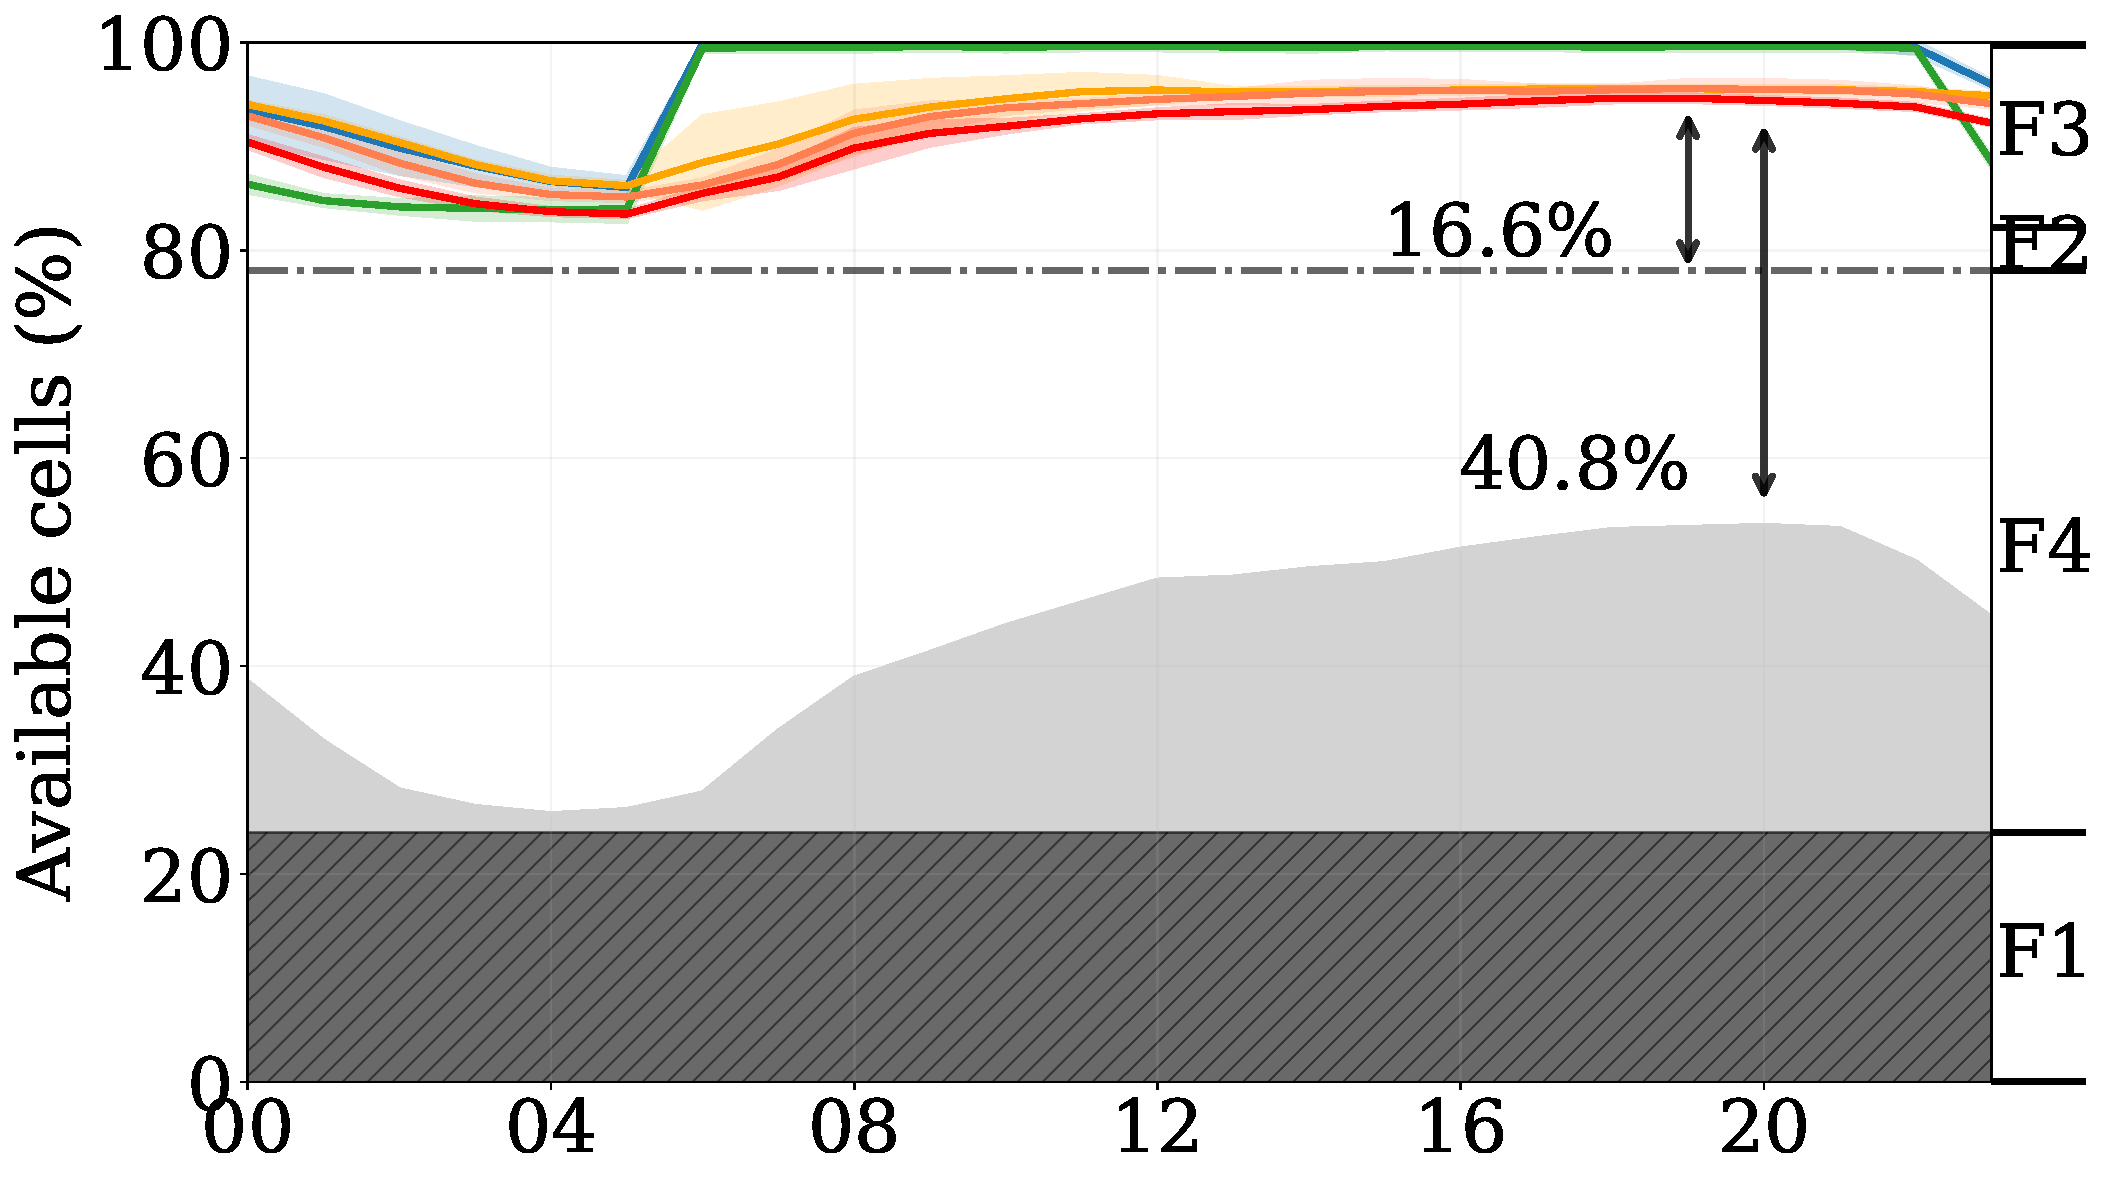
\includegraphics[width=.5\columnwidth]{images/availability/network_usage/fraction_of_available_antennas_north_london.pdf}}
    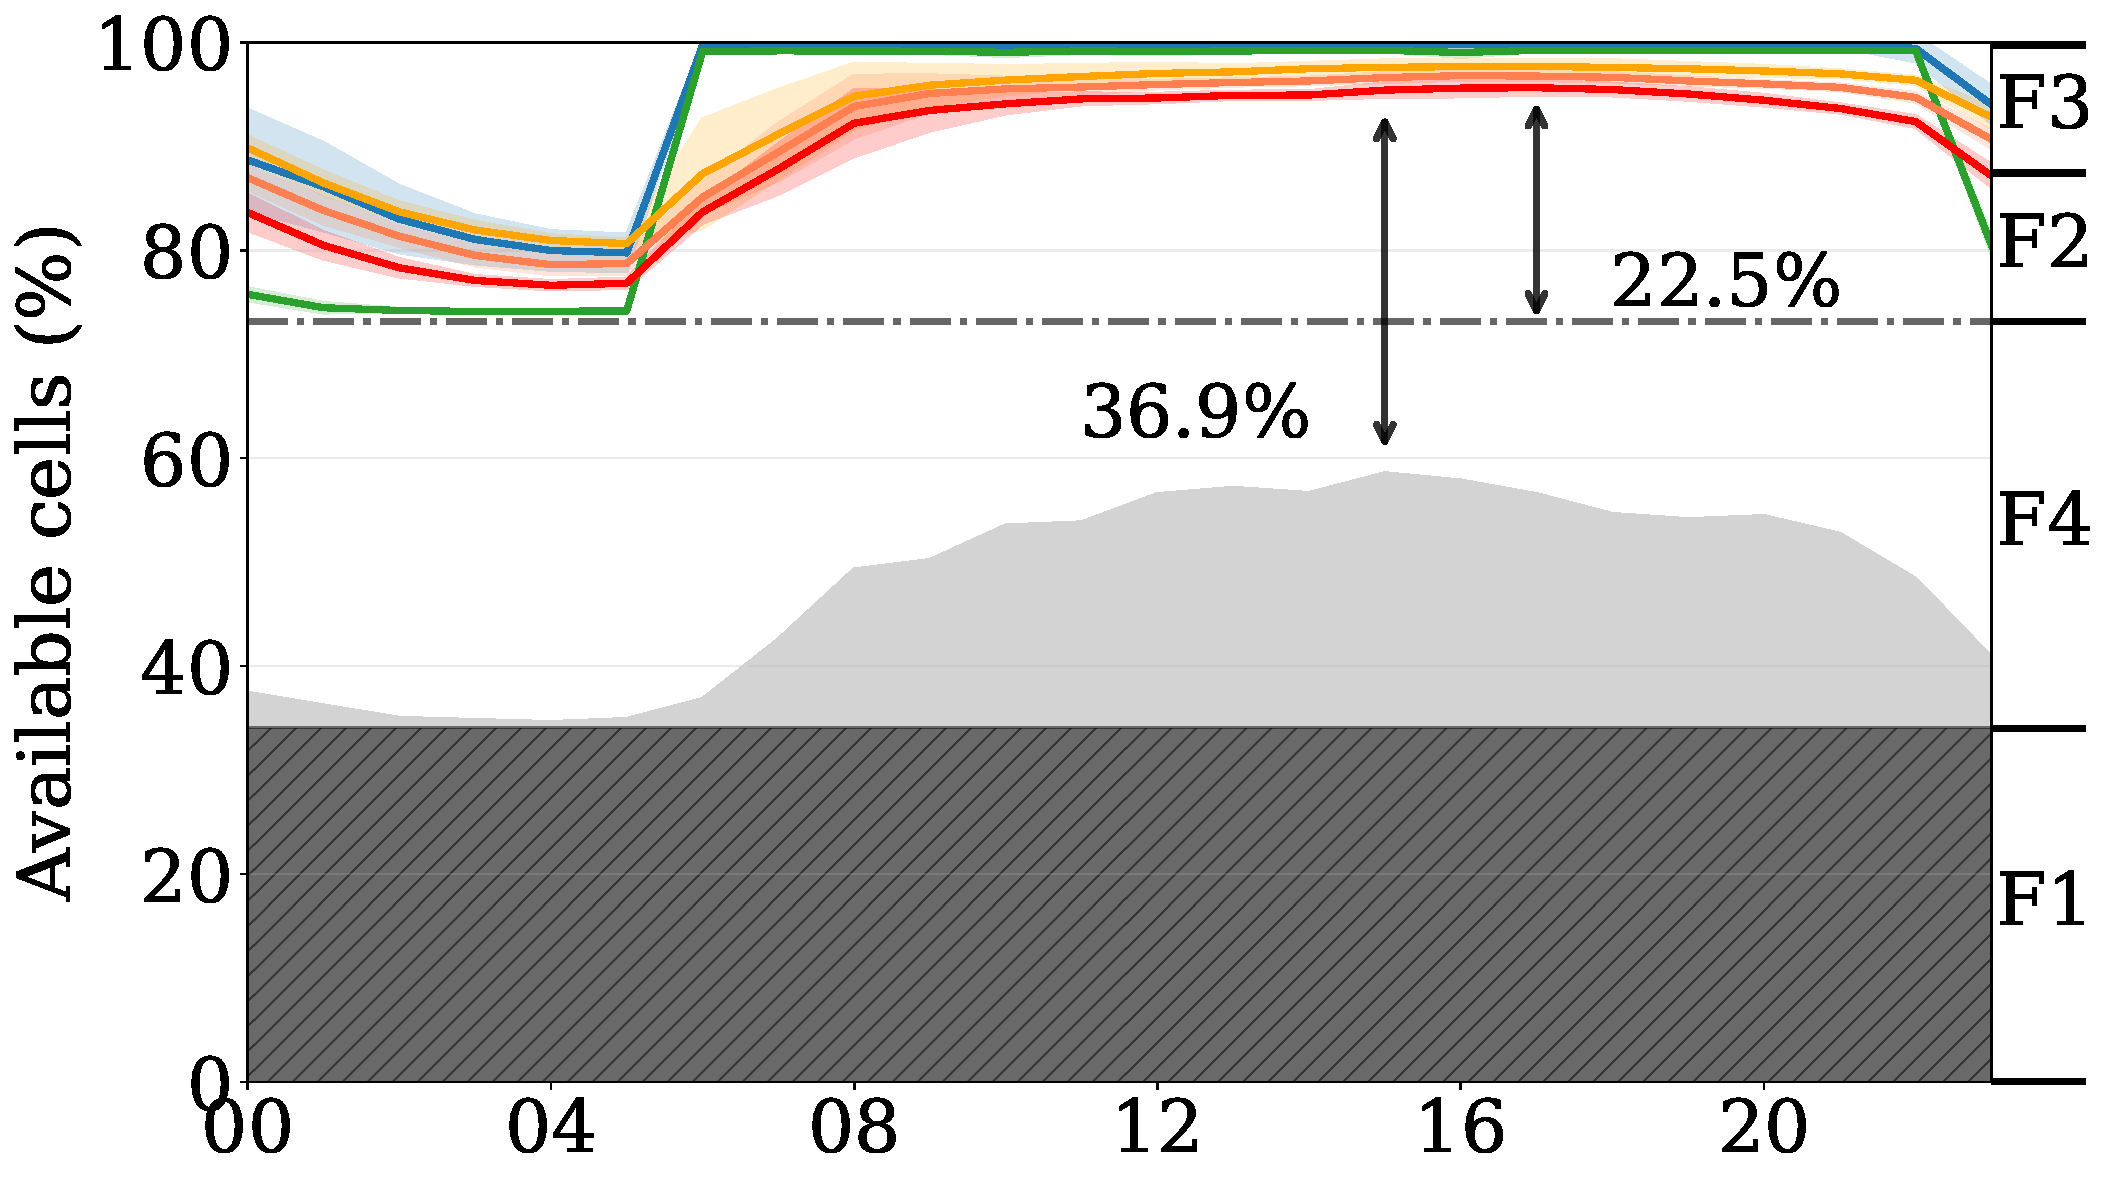
\includegraphics[width=.75\columnwidth]{images/availability/network_usage/fraction_of_available_antennas_southeast.pdf}
    \vspace{-4pt}
    \caption{\small Percentage of available cells on an hourly basis for each strategy, compared to the fraction of capacity cells, coverage cells, and the cells theoretically needed to meet the current demand. The curves refer to the Sparse region. 
    % \js{can we remove the subfigure here? "Sparse region" is already specified in the caption} 
    % \js{modify the legend "Antennas to meet the demand" -$>$ "Cells to meet the demand"}
    % \mf{yes, but F1, \dots, F4 are still hard to read, maybe you can remove the grey backgrounds and just have normal labels and out-tics at the boundaries of the frequencies on the y2 axis?}\om{like this?}
    % \js{Y axis: Available cells}
    \label{fig:percentage_available_antennas_coverage_demand}}
    \vspace{-15pt}
\end{figure}

We now discuss the multiple implications of our study for practical energy savings in production mobile networks.

\textbf{Avenues for improvement in RAN sustainability.} Our results clearly show that the use of a single pair of ON/OFF thresholds for all regions is sub-optimal. Fixed thresholds that are indiscriminately applied to a whole RAN deployment, even in the same TAC, risk being overly conservative for some cells and just disruptive for others, as suggested by the diversity seen in Figure~\ref{fig:energy_saving_impact_kpi_class}. A more effective approach could involve setting specific thresholds at the power group level or grouping cells into different clusters with various treatments, which could potentially help yield greater energy savings while keeping an unnoticeable impact on QoE. 
These tailor-made thresholds could also be dynamically updated using machine learning techniques. Finally, incorporating information about the load of neighboring cells and sites into the decision process could enhance the effectiveness of cell sleep strategies.

\textbf{Limited energy savings overall}.  
Throughout the paper, we have focused on energy savings at the capacity cells that are allowed to go in sleep mode. We now take a broader view and put the energy savings presented in previous sections in the context of the whole RAN deployments in the target areas.

Figure~\ref{fig:percentage_available_antennas_coverage_demand} shows $(i)$~the percentage of available cells for each strategy along the day (hourly intervals), including capacity and coverage cells, $(ii)$~the theoretical percentage of cells required to meet the ongoing traffic demand in the region, $(iii)$~the percentage of capacity cells subject to energy saving strategies, and $(iv)$~the percentage of coverage cells, which ensure service along the region. There is a notable gap between available cells, the fraction needed to meet demand, and coverage cells. The Night-strict strategy comes closest to putting all capacity cells to sleep at night, while during the day, the Full-strict strategy is more effective, displaying a similar behavior to other full-day strategies. These results indicate that while these strategies reduce energy consumption, they are far from optimal and could be significantly improved. %\jo{why is this happening? are the threshold too conservative?}

Furthermore, Figure~\ref{fig:energy_saving_full_regions} shows the total energy saving (in \% of improvement over the benchmark model), considering all cells deployed in each region~--~including both coverage and capacity cells. Note that the previous results in Figure~\ref{fig:percentage_energy_saving_capacity_boosters} considered only savings on capacity cells, which are the ones affected by the cell sleep policies tested by the MNO. These results of total savings reveal more reduced savings at the RAN level, which evidences the conservative nature of current strategies deployed nowadays in production networks. %\jo{again, why does this happens, and also what could be done in the future to improve it? e.g., threshold per antenna based on ML?}

\begin{figure}
    \centering
    \vspace*{-4pt}
    \subfloat[Dense region]{
\includegraphics[width=.45\columnwidth]{images/energy/energy_saving/whole_network/saving_percentage_north_london.pdf}}
    \hspace{5pt}
    \subfloat[Sparse region]{
\includegraphics[width=.45\columnwidth]{images/energy/energy_saving/whole_network/saving_percentage_southeast.pdf}}
    \vspace{-4pt}
    \caption{\small Total energy saving in the two regions. Although there is a gain in savings as strategies become more aggressive, the total savings are significantly reduced w.r.t. those observed on capacity cells.}
    \label{fig:energy_saving_full_regions}
    \vspace{-15pt}
\end{figure}

%Figure~\ref{fig:energy_saving_full_regions} shows the overall savings percentage of the total network consumption in each region that is saved by each strategy, revealing that these savings are relatively small overall, confirming that these strategies are extremely conservative. \js{Compare it with Fig~\ref{fig:percentage_energy_saving_capacity_boosters}}

 \textbf{Energy savings do not imply $\text{CO}_2$ savings}. Although this work primarily focuses on energy savings, we also evaluated the impact on $\text{CO}_2$ emissions, specifically Scope 2 emissions as defined by the GHG Protocol \cite{GHG2023}. The Greenhouse Gas (GHG) Protocol categorizes emissions into three scopes: Scope 1 includes direct emissions from company activities like burning fuels; Scope 2 covers indirect emissions from purchased energy, such as electricity from the grid; and Scope 3 encompasses all other indirect emissions across the value chain. Our threshold-based energy-saving policies directly influence Scope 2 emissions, measured in grams of $\text{CO}_2$ equivalent per kilowatt-hour (g$\text{CO}_2$eq/kWh). While reducing energy consumption decreases $\text{CO}_2$ emissions, the alignment between energy savings and emission reductions is not always straightforward. Energy-saving policies focus on reducing energy use without considering the carbon intensity of energy production. In the country under study, carbon fuels constitute a significant part of the energy grid, affecting the overall impact of these policies. Figure~\ref{fig:carbon_emission_energy_consumption} shows the carbon emission in the country during the week of the Night-strict trial. Although there is a regular pattern where emissions decrease overnight and increase over daylight hours, there is a significant variability along the days that we can exploit to achieve more carbon-efficient policies. %in order to also minimize the $\text{CO}_2$ emission if the energy saving strategies considered CO2 hourly estimations into their methodology.

 \begin{figure}
    % \vspace*{-10pt}
    \centering
    %\subfloat{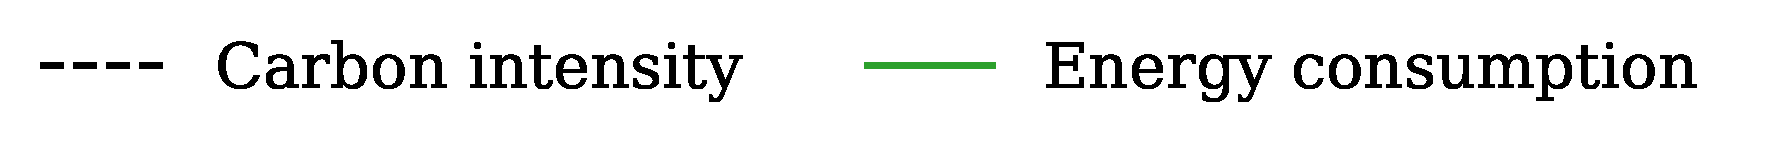
\includegraphics[width=.8\columnwidth]{images/co2/capacity_booster/emissions_vs_energy_consumption_southeast_Baseline_legend.pdf}}
    \setcounter{subfigure}{0}
    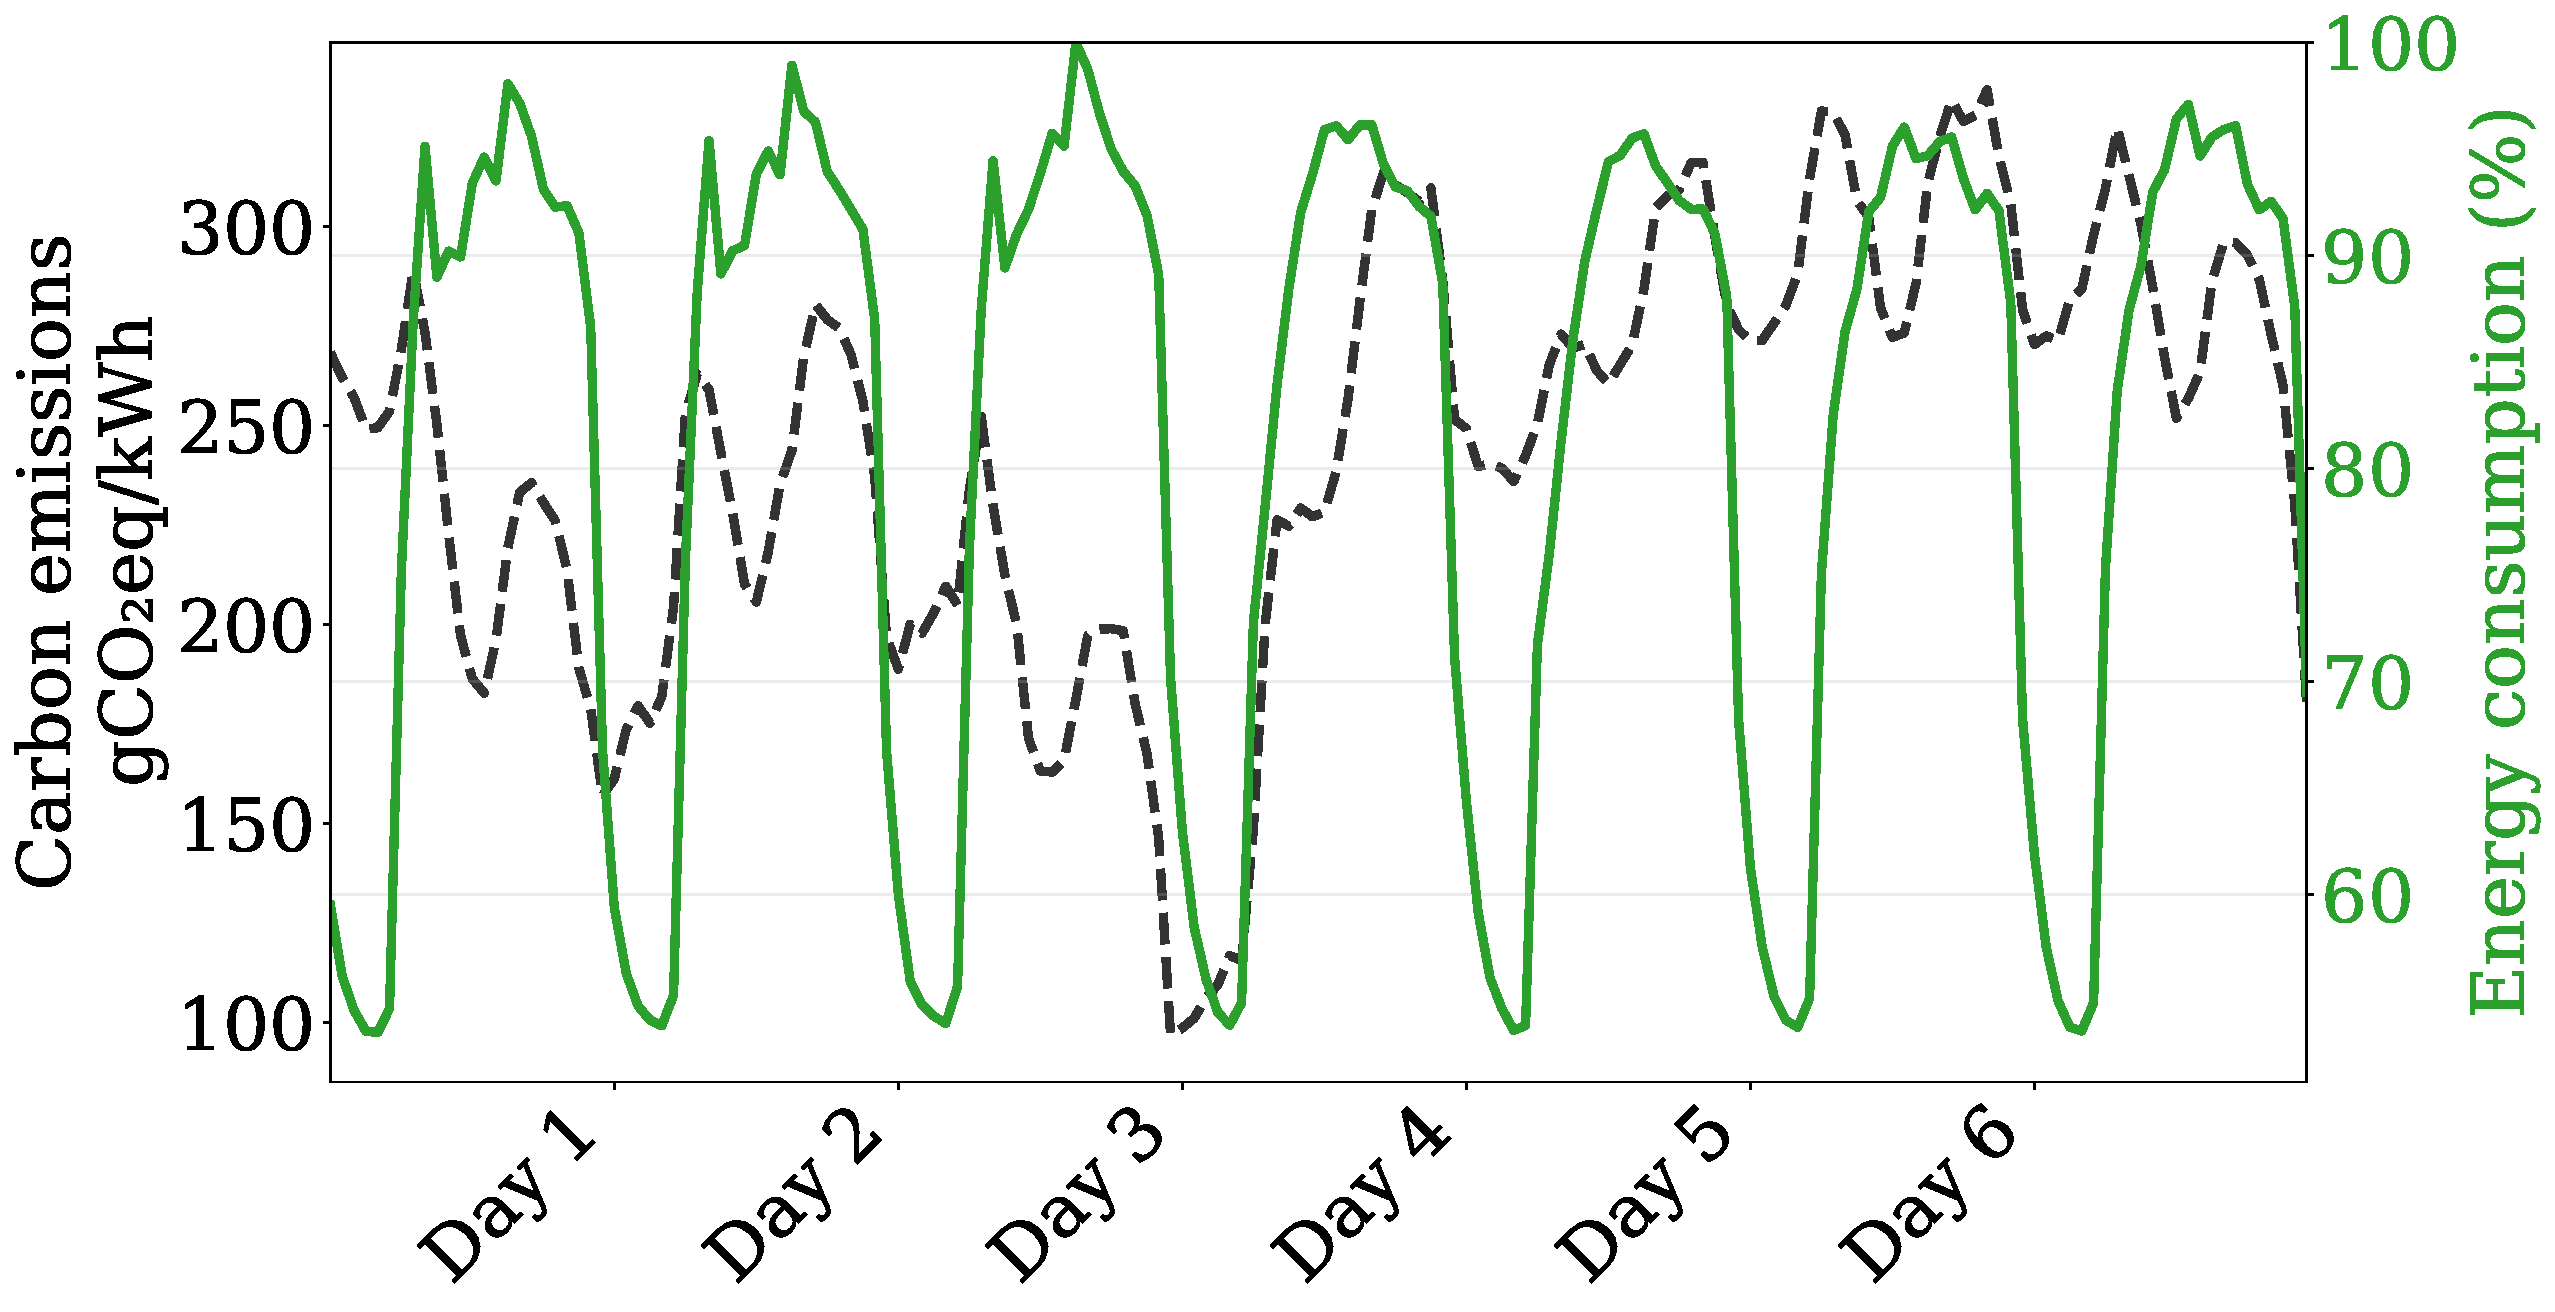
\includegraphics[width=.75\columnwidth]{images/co2/capacity_booster/emissions_vs_energy_consumption_southeast_Baseline.pdf}
    \vspace*{-4pt}
    \caption{\small Estimated carbon intensity in g$\text{CO}_2$eq/kWh and energy consumption in the Sparse region during the week of the second trial. Energy consumption values are normalized with respect to the maximum hourly consumption for confidentiality reasons.
    \label{fig:carbon_emission_energy_consumption}}
    \vspace{-15pt}
\end{figure}